%
% File acl2020.tex
%
%% Based on the style files for ACL 2020, which were
%% Based on the style files for ACL 2018, NAACL 2018/19, which were
%% Based on the style files for ACL-2015, with some improvements
%%  taken from the NAACL-2016 style
%% Based on the style files for ACL-2014, which were, in turn,
%% based on ACL-2013, ACL-2012, ACL-2011, ACL-2010, ACL-IJCNLP-2009,
%% EACL-2009, IJCNLP-2008...
%% Based on the style files for EACL 2006 by 
%%e.agirre@ehu.es or Sergi.Balari@uab.es
%% and that of ACL 08 by Joakim Nivre and Noah Smith

\documentclass[11pt,a4paper]{article}
\usepackage[hyperref]{acl2020}

\usepackage{amsmath}
\usepackage{amsfonts}
\usepackage{amssymb}
\usepackage{booktabs}
\usepackage{color, colortbl}
\usepackage{enumitem}
\usepackage{graphicx}
\usepackage{hyperref}
\usepackage[latin1]{inputenc}
\usepackage{latexsym}
\usepackage{multirow}
\usepackage{times}
\usepackage{url}
\usepackage{xcolor}
\usepackage{xspace}

\renewcommand{\UrlFont}{\ttfamily\small}

%\usepackage{microtype}

%\aclfinalcopy % Uncomment this line for the final submission
%\def\aclpaperid{***} %  Enter the acl Paper ID here

%\setlength\titlebox{5cm}
% You can expand the titlebox if you need extra space
% to show all the authors. Please do not make the titlebox
% smaller than 5cm (the original size); we will check this
% in the camera-ready version and ask you to change it back.

\newcommand{\sz}[1]{\textcolor{blue}{\emph{//sz: #1//}}}
\newcommand{\gbt}[1]{\textcolor{orange}{\emph{//gbt: #1//}}}
\newcommand{\cs}[1]{\textcolor{green!60!black}{\emph{//cs: #1//}}}
\newcommand{\mw}[1]{\textcolor{orange!60!black}{\emph{//mw: #1//}}}

% To streamline frequently used terms:
\newcommand{\langvis}{language\ \&\ vision\xspace}
\newcommand{\lv}{L\&V\xspace}
\newcommand{\mn}{ManyNames\xspace}
\newcommand{\vg}{VisualGenome\xspace}

\newcommand{\cat}[1]{\textsc{#1}}
\newcommand{\name}[1]{\textsl{#1}}

% Terms that need to be replaced throughout the paper by more appropriate ones:
\newcommand{\arbitrary}{arbitrary$\rightarrow$?\xspace}


\title{Supplementary Material}

\author{First Author \\
	Affiliation / Address line 1 \\
	Affiliation / Address line 2 \\
	Affiliation / Address line 3 \\
	\texttt{email@domain} \\\And
	Second Author \\
	Affiliation / Address line 1 \\
	Affiliation / Address line 2 \\
	Affiliation / Address line 3 \\
	\texttt{email@domain} \\}

\date{}

\begin{document}


\section{Verification Procedure with AMT}
\label{sec:verif}
\begin{figure*}[t]
	\centering
	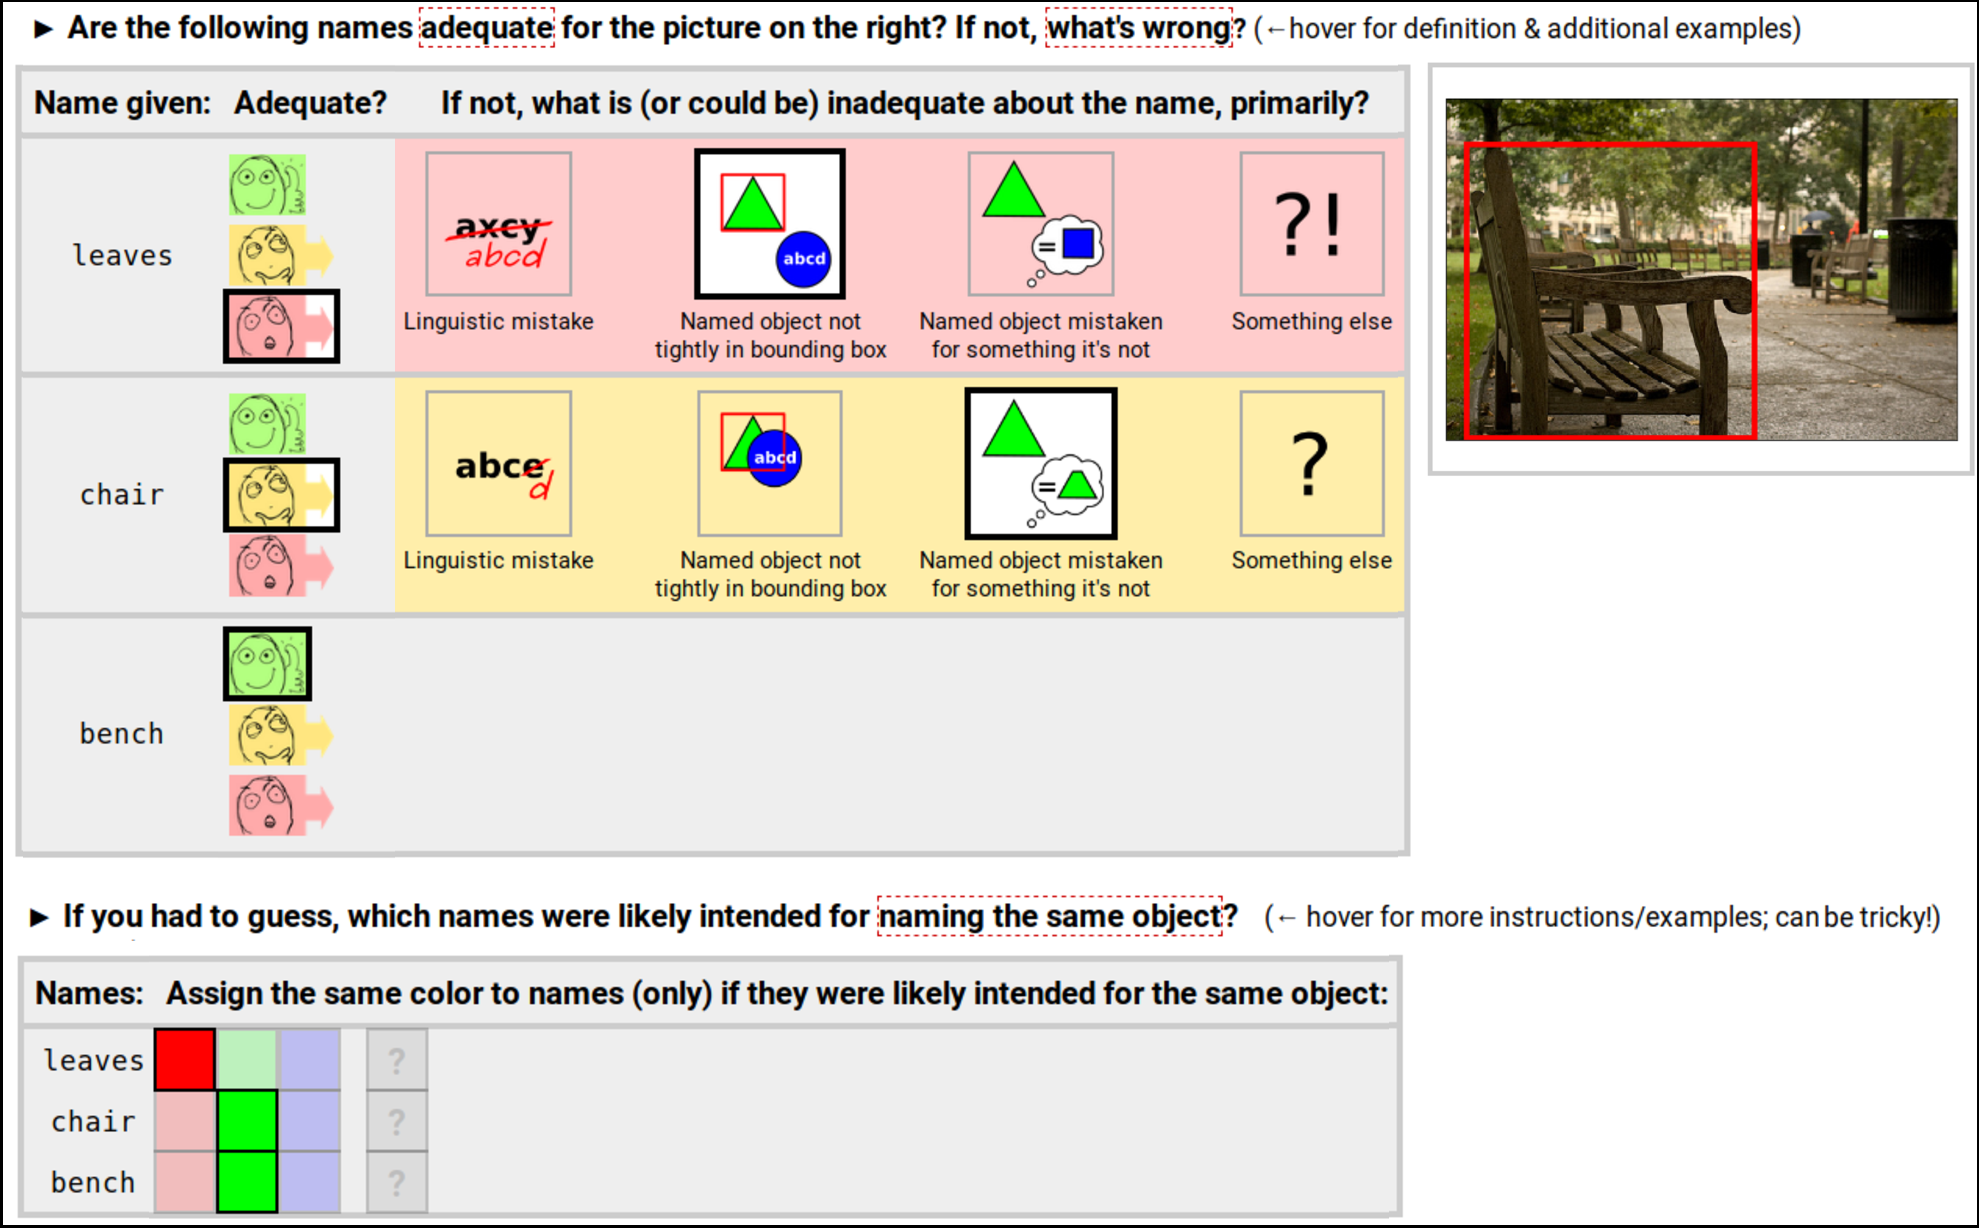
\includegraphics[width=\textwidth]{images/verification-interface.pdf}
	\caption{A screenshot of our verification task interface. Up to ten names could be shown for an image in this way (the number of available colors in the second task would increase accordingly).}
	\label{fig:verification-interface}
\end{figure*}

\cs{The text is is just copied from the main, it needs to be adapted here.}
We provided (and clarified by means of explanation and visual examples) the following definition: \textit{a name is ``adequate'' if there is an object in the image, whose visible parts are tightly circumscribed by the red bounding box, that one could reasonably call by that name}.
When the participant selected slightly or totally inadequate, four additional icons would appear to indicate the type of inadequacy: ``linguistic mistake'', ``named object not tightly in bounding box'', ``named object mistaken for something it's not'', and ``something else''.
We provided detailed instructions and examples at the top, as well as informative hover texts on all the buttons.

\bibliographystyle{acl_natbib}
\bibliography{naming}
\end{document}